\documentclass{article}
\usepackage{float}
\usepackage{graphicx}
\usepackage{cleveref}
\usepackage{hyperref}

\begin{document}

\title{Project in Advanced Multiprocessor Programming}
\author{Simon Mayer - 11776870, Krasimir Kanev - 12345086}
\maketitle
\tableofcontents
\newpage
\section{Benchmark}

The benchmark functionality stretches over several files. 
Most of the overhead work is done in the python files which are called from the make targets. 
Here the desired parameters are cycled through. With a specific set of the parameters a single benchmark instance is performed by calling the static C library benchmark.
The benchmark with a single set of parameters is repeated in this way for the specified amount of times.
After finishing all thread number variations of an implementation, the results are averaged over the repetitions and written to the according file.
The fields that are collected are:
\begin{enumerate}
    \item n\_threads: The number of threads this datapoint was recorded at
    \item n\_successfull\_adds: The sum of number of successful add (insert) operations over all threads
    \item n\_failed\_adds: The sum of number of failed add (insert) operations over all threads (key was already in set)
    \item n\_successfull\_contains: The sum of number of contains (find) operations over all threads where the key was in the list
    \item n\_failed\_contains: The sum of number of contains (find) operations over all threads where the key was not present
    \item n\_successfull\_removes: The sum of number of successful remove (erase) operations over all threads
    \item n\_failed\_removes: The sum of number of failed remove (erase) operations over all threads (key was not in set)
    \item total\_operations: Sum of all operations performed over all threads
    \item max\_thread\_time: The maximum time any of the threads spent on the operations (described in more detail below)
    \item throughput: Calculated by dividing total\_operations by max\_thread\_time
\end{enumerate}

In the C library "benchmark" the functions of the respective skip list implementations are called.
After creating the list, it is pre-filled and the counters are initialized.
For the concurrent implementations, the OpenMP parallel regions then follow where the actual operations are performed. The next key is chosen based on the desired strategy and the type of operation is randomly chosen based on the mix of operations that was supplied.
Directly before and after the operations a timestamp is taken with the POSIX standard function "clock\_gettime" which the difference of is added to the threads CPU time. We decided to do this to exclude the time it takes to select keys and operation kind from our measurements.
When the pre-defined measurement duration is elapsed, the experiment stops and OMP's reduction clause adds up the results of each thread.
The results are then passed back to the python execution, where they are handled as described above.

Throughout the project, we used the following parameters for our benchmark measurements:

\begin{enumerate}
    \item op-mix-1: add:0.1, del:0.1, find:0.8
    \item op-mix-2: add:0.4, del:0.4, find:0.2
    \item strat-1: random access
    \item strat-2: uniquely random access
    \item overlap-1: common key-space for all threads
    \item overlap-2: disjoint key-space for threads
\end{enumerate}
\begin{table}[H]
    \centerline{
    \begin{tabular}{c|c|c|c|c}
        Parameter & parameters1\_1s & parameters1\_5s & parameters2\_1s & parameters2\_5s\\
        Operation mix &  op-mix-1 & op-mix-1 & op-mix-2 & op-mix-2 \\
        Selection strategy & strat-1 & strat-1 & strat-2 & strat-2 \\
        Key overlap & overlap-1 & overlap-1 & overlap-2 & overlap-2\\
        Measurement interval & 1 second & 5 seconds & 1 second & 5 seconds\\
    \end{tabular}
    }
    \caption{parameter table}
    \label{tab:parameters}
\end{table}
\newpage
\section{Sequential skip list}


The node structure in the skip list is designed to enable efficient traversal and operations within an ordered list. Each node consists of a key, which serves as the value or identifier for ordering and searching, and a dynamically allocated array of pointers. These pointers connect to subsequent nodes at different levels, allowing the skip list to skip over sections of the list and perform operations more quickly.

The implementation of the skip list revolves around the principles of multi-level linking and probabilistic balancing. Nodes are connected at various levels, with higher levels acting as shortcuts for fast traversal. The height of a node, which determines the number of levels it participates in, is assigned probabilistically using a random number generator. The implementation relies on the \texttt{drand48} family of functions for this purpose, ensuring that node heights are distributed according to the specified probability factor. 

Core operations in the skip list include search, insertion, and deletion. Searches begin at the highest level of the list and proceed downward, skipping over unnecessary nodes to quickly locate the desired key. Insertions involve creating a new node with a height determined probabilistically using \texttt{drand48\_r}, then linking the node at the appropriate levels while preserving the structure of the list. Deletions are handled by unlinking nodes from all levels they participate in, ensuring that the skip list remains consistent and orderly.

\vspace{5mm}
The structure of a single node comprises the nodes key (an int), a pointer to optional data (void*, not used in benchmark) and an array of pointers to the next node. All nodes present in the list are linked at level 0, the upper levels are linked depending on the height of the node.

Besides the head node, a sequential skip list structure also contains information about the highest level nodes are linked at, the probability at which higher levels are chosen and the accepted key range.
To maintain consistent and reproducible behavior, a \texttt{random\_state} structure is included in the skip list structure. This is used to keep state for the random number generator. During initialization, the \texttt{srand48\_r} function is called with a user-specified seed to set up this random state, and the \texttt{drand48\_r} function is subsequently used to generate random numbers during operations such as node height determination.

\subsection{Sequential skiplist benchmark results}

A plot of the results of benchmark runs with different parameters can be observed in \ref{fig:sequential_plot}.

\begin{figure}[ht!]
  \centering
  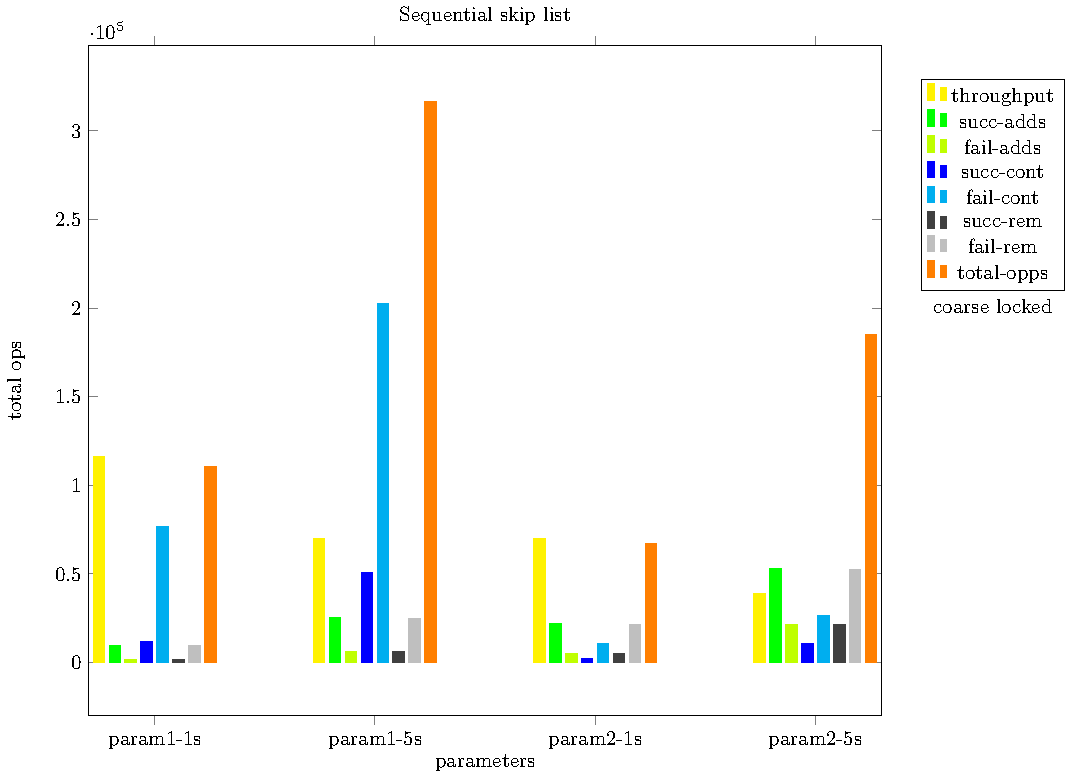
\includegraphics[width=\textwidth]{../plots/sequential_throughput.pdf}
  \caption{Performance of sequential implementation under different parameters}
  \label{fig:sequential_plot}
\end{figure}

We can see that for a specific parameter set the operation counters scale with the time difference of a 1 second measurement interval to a 5 second measurement interval. The throughput, which should be indifferent to the interval, is decreasing with the longer experiments.
For parameters1 (param1 in the graph) we see that the high amount of contain queries fails most of the time as there are not that many elements in the list at any time in relation to the key-space.
This sparse environment is also the reason why most add operations succeed and most remove operations fail in our random access pattern.

\newpage

\section{Coarse skiplist}

The implementation is largely identical to the sequential one, however the coarse-list structure contains one lock that is set and unset by every concurrent operation, granting exclusive access to the nodes of the list.

\subsection{Coarse skiplist benchmark results}

The results from the benchmark are visualized in the following plots below:
\begin{enumerate}
    \item \textbf{Total throughput}
    \begin{figure}[H]
        \centering
        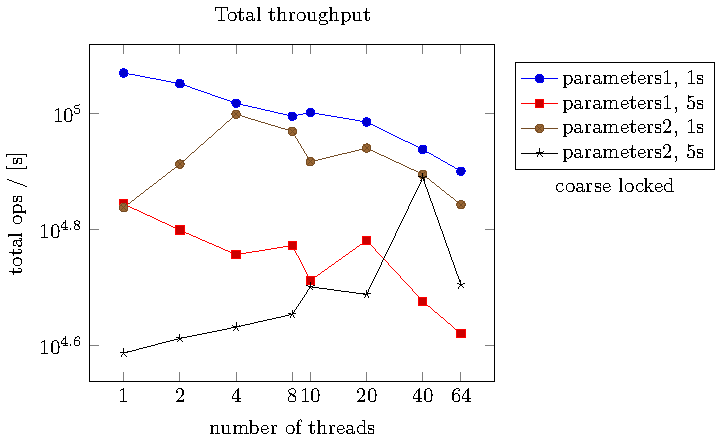
\includegraphics{../plots/coarse_throughput.pdf}
        \caption{ The results demonstrate higher throughput for parameters1 configuration due to reduced contention, while both workloads plateau at higher thread counts, reflecting the scalability limitations of coarse-grained locking.}
       
        \label{fig:coarse_skiplist_throughput}
    \end{figure}
The throughput plot shows that the execution with parameters1 config outperforms parameter2 config due to simpler operations. However, the global lock imposes a hard throughput ceiling, with performance even decreasing with higher thread counts regardless of the workload or measurement interval. This highlights the fundamental limitations of coarse-grained locking in multi-threaded scenarios.

    \item \textbf{Total operation per thread}
    \begin{figure}[H]
        \centering
        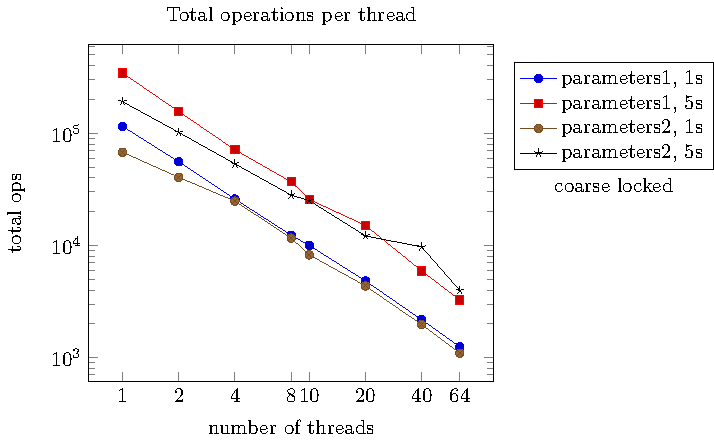
\includegraphics{../plots/coarse_per_thread.pdf}
        \caption{The plot highlights the impact of workload composition and lock contention on per-thread performance as thread count increases.}
        \label{fig:coarse_ops_per_thread}
    \end{figure}
   The plot reveals that per-thread operations decrease as the number of threads increases, due to contention caused by the coarse-grained lock. The parameter1 configuration achieves a higher number of per-thread operation compared to the parameter2 configuration, due to the simpler operations. The trends are consistent between 1-second and 5-second execution intervals, indicating that the system stabilizes quickly. At higher thread counts, the global lock becomes a bottleneck, limiting scalability and causing a sharper decline in per-thread performance.

    
\end{enumerate}

\newpage

\section{Lazy skip list}

The implementation is very similar to what was presented in the lecture.
Instead of a global lock for all operations, each node possesses its own lock and a marked-for-deletion and fully-linked flag. For optimization purposes the nodes also record their height.
The add and remove functions only lock those nodes that are necessary for performing the insertion or deletion while the contains operation even is wait-free.

Unfortunately, as we will later also see in the benchmark, we had problems with liveness in our lazy skip list implementation.
For parameters2 the benchmark would not terminate above a thread count of 10.

\subsection{Lazy skip list benchmark results}

\begin{enumerate}
    \item \textbf{Total throughput}
    \begin{figure}[H]
        \centering
        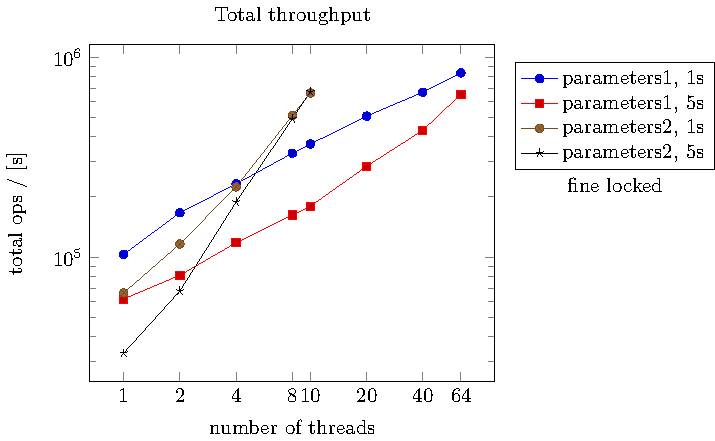
\includegraphics{../plots/fine_throughput.pdf}
        \caption{ Throughput measurements for the lazy skip list}
       
        \label{fig:fine_skiplist_throughput}
    \end{figure}
    We can see similar scaling with the thread count for the runs with parameters1, regardless of the measurement interval. As mentioned before the measurement with parameters2 did not terminate for thread count higher than 10.
    However the performance does not experience a bottleneck because of contention as observed in the coarse skip list implementation.
    \item \textbf{Total operations per thread}
    \begin{figure}[H]
        \centering
        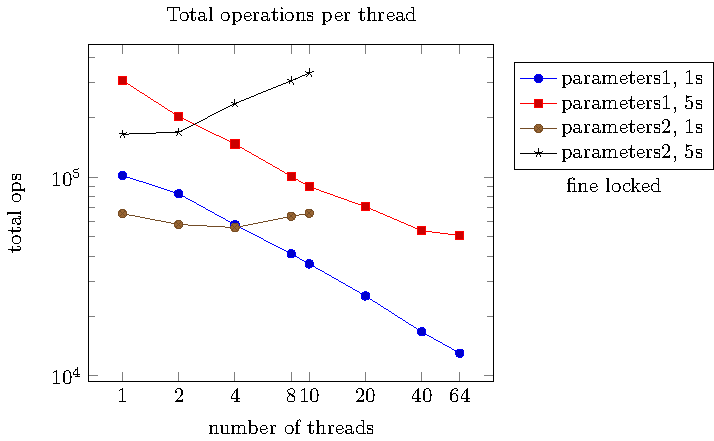
\includegraphics{../plots/fine_per_thread.pdf}
        \caption{ Total operations per thread for the lazy skip}       
        \label{fig:fine_skiplist_per_thread}
    \end{figure}
    We can speculate about what might be happening by considering both plots. Throughput and operations per thread are both increasing with thread count for parameters2. Since the amount of add operations is higher with this configuration, we might run out of memory and the threads are stuck in the add function.
    The lines for parameters1 show the expected behavior: decreasing operations per thread for a higher thread count.
\end{enumerate}

\newpage

\section{Lock-free skip list}
At the heart of this implementation lies the extensive use of atomic operations, thread coordination strategies, and a carefully crafted design that ensures progress and consistency.

Atomic operations are the cornerstone of the lock-free skip list, enabling thread-safe updates to shared variables. The \texttt{\_\_atomic\_compare\_exchange} primitive CAS plays a critical role. It allows threads to compare the current value of a variable with an expected value and update it only if the two match, ensuring that updates are atomic and consistent. This mechanism is widely used to modify pointers during operations like insertion or deletion. Alongside CAS, other atomic primitives, such as \texttt{\_\_atomic\_fetch\_add} and \texttt{\_\_atomic\_fetch\_sub}, are employed for incrementing or decrementing counters. These operations, combined with atomic load and store functions, ensure that threads can access and update shared variables without race conditions. All these operations are configured with relaxed memory ordering (\texttt{\_\_ATOMIC\_RELAXED}), which optimizes performance by reducing synchronization overhead while maintaining the correctness of the data structure.

Thread coordination in the skip list is achieved through non-blocking mechanisms. The implementation uses \texttt{sched\_yield()} to allow a thread to relinquish its execution time when it detects contention, enabling other threads to proceed. This approach minimizes busy-waiting and promotes fairness among threads. When CAS operations fail due to concurrent modifications, the skip list relies on retry logic, where threads reattempt the operation using the updated state of the data structure. This contention-handling strategy ensures that operations eventually succeed without blocking other threads.

Moreover, each node in the skip list maintains an array of pointers corresponding to its levels. Updates to these pointers are performed level-by-level, limiting the scope of contention and allowing threads to work independently on different parts of the structure. 

In addition, all critical updates to pointers or node states are performed using CAS. In order to handle deletions safely, nodes are first marked as logically deleted before being physically removed. This prevents inconsistencies, as a node being traversed by one thread might simultaneously be targeted for deletion by another. This two-step deletion process, combined with atomic pointer updates, ensures that the structure remains consistent and robust.

\newpage
\subsection{Lock-free skiplist benchmark results}
The results from the benchmark are visualized in the following plots below:
\begin{enumerate}
    \item \textbf{Total throughput}
    \begin{figure}[H]
        \centering
        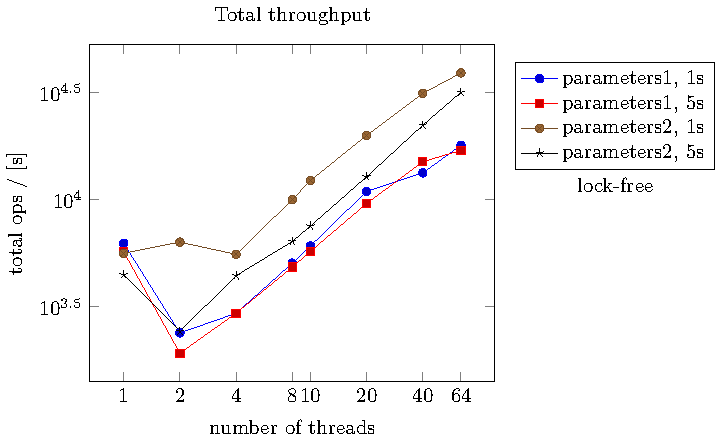
\includegraphics{../plots/lock_free_throughput.pdf}
        \caption{The graph demonstrates scalability with increasing thread count and highlights the impact of parameter tuning on system performance.}
       
        \label{fig:lock_free_throughput}
    \end{figure}
    Both configurations show an initial decrease in throughput as the number of threads grows. Performance takes a big hit when going from a single thread to only a small number of parallel ones. This shows the cost of concurrency in this implementation. However with a larger amount of threads the implementation begins to gain performance again over all parameter configurations. 

    \item \textbf{Total operation per thread}
    \begin{figure}[H]
        \centering
        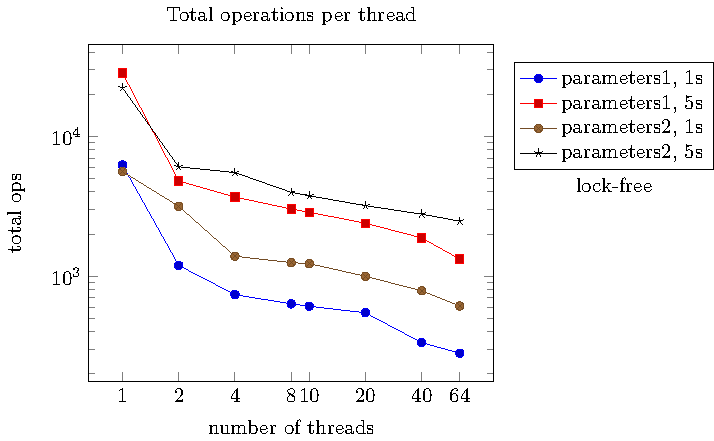
\includegraphics{../plots/lock_free_per_thread.pdf}
        \caption{The plot highlights the effects of workload composition and thread contention on per-thread performance as the thread count increases.}
        \label{fig:lock_free_ops_per_thread}
    \end{figure}
    The plot shows the per-thread throughput of a lock-free system as the number of threads increases, with workloads defined by two configurations: parameter1 and parameter2. As thread count grows, per-thread throughput decreases due to increasing contention and the system's overall throughput plateauing. 
    Interestingly in this metric, as well as in \ref{fig:lock_free_throughput} the parameters2 configuration leads to a better performance, highlighting the advantage of disjoint key-spaces.

    
\end{enumerate}

\newpage
\section{Benchmark results comparison}


Below are shown comparison results from the benchmark with the subjected skiplist implmentations and various parameter configurations:
    \begin{figure}[H]
        \centering
        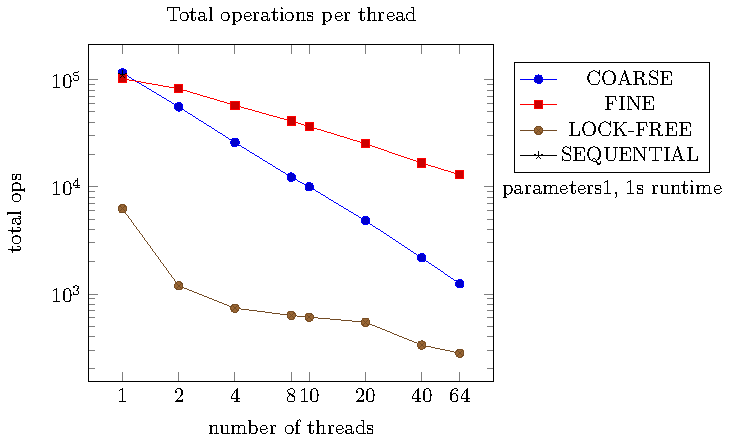
\includegraphics{../plots/parameters1_1s_per_thread.pdf}
        \caption{Configuration parameters1 TOPS per thread,1s execution time}
       
        \label{fig:parameters1_1s_per_thread}
    \end{figure}

    \begin{figure}[H]
        \centering
        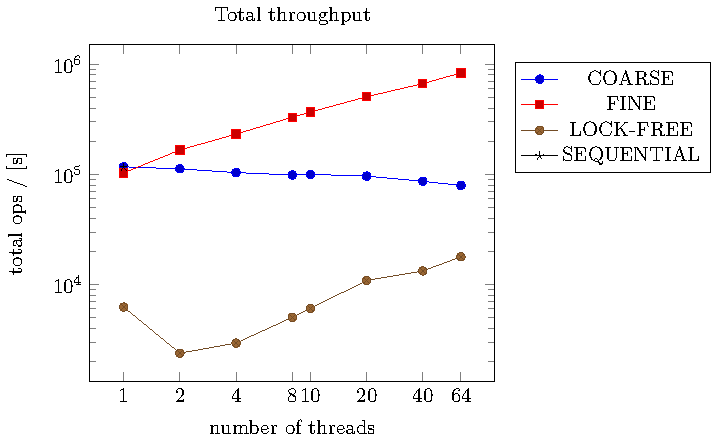
\includegraphics{../plots/parameters1_1s_throughput.pdf}
        \caption{Configuration parameters1 Throughput, 1s execution time}
        \label{fig:parameters1_1s_throughput}
    \end{figure}

    \begin{figure}[H]
        \centering
        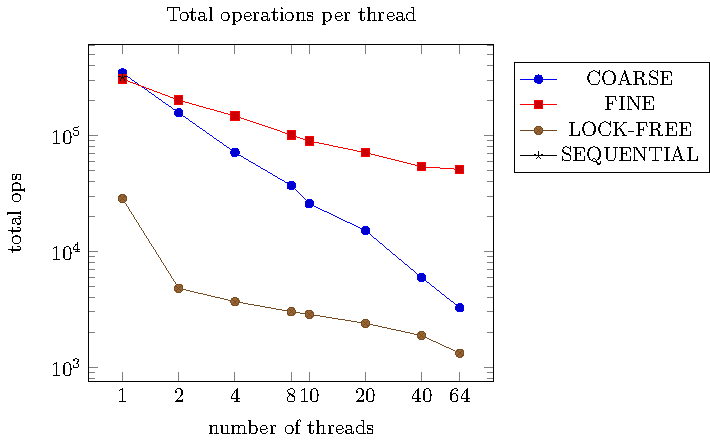
\includegraphics{../plots/parameters1_5s_per_thread.pdf}
        \caption{Configuration parameters1 TOPS per thread,5s execution time}
       
        \label{fig:parameters1_5s_per_thread}
    \end{figure}

    \begin{figure}[H]
        \centering
        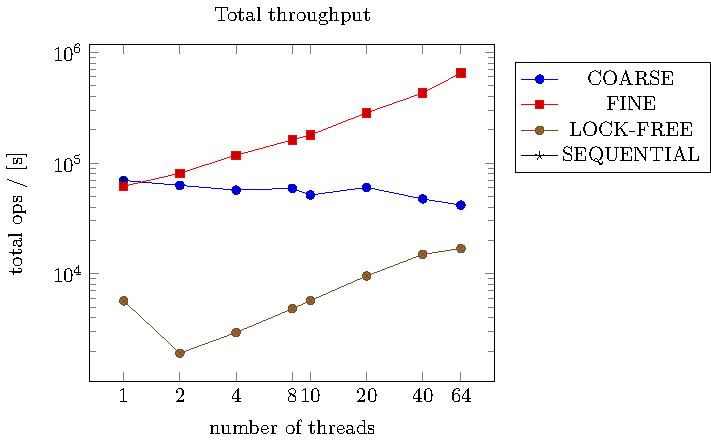
\includegraphics{../plots/parameters1_5s_throughput.pdf}
        \caption{Configuration parameters1 Throughput, 5s execution time}
        \label{fig:parameters1_5s_throughput}
    \end{figure}

    \begin{figure}[H]
        \centering
        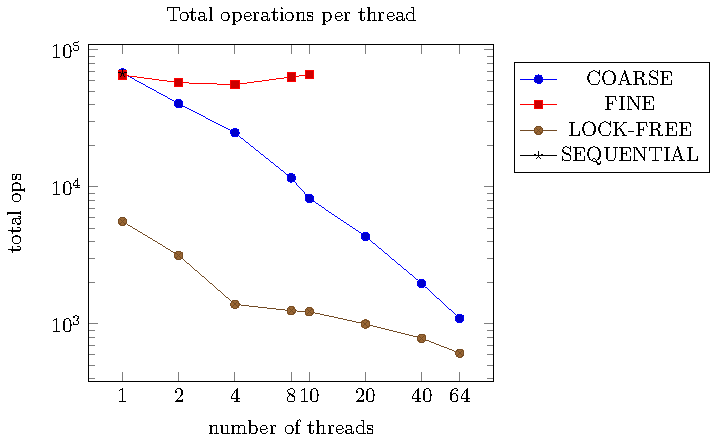
\includegraphics{../plots/parameters2_1s_per_thread.pdf}
        \caption{Configuration parameters2 TOPS per thread,1s execution time}
       
        \label{fig:parameters2_1s_per_thread}
    \end{figure}

    \begin{figure}[H]
        \centering
        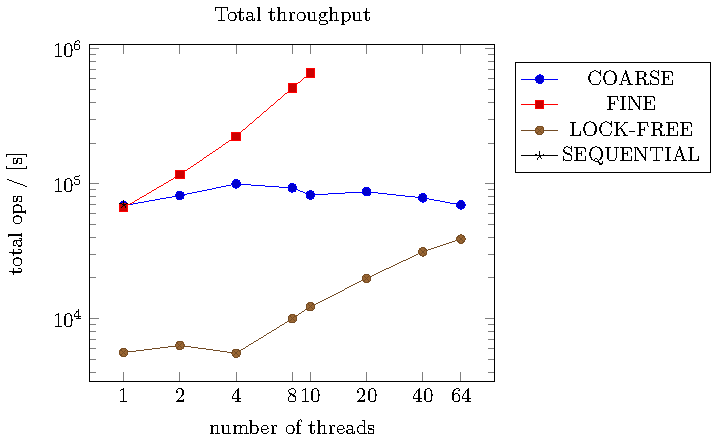
\includegraphics{../plots/parameters2_1s_throughput.pdf}
        \caption{Configuration parameters2 Throughput, 1s execution time.}
        \label{fig:larameters1_1s_throughput}
    \end{figure}

    \begin{figure}[H]
        \centering
        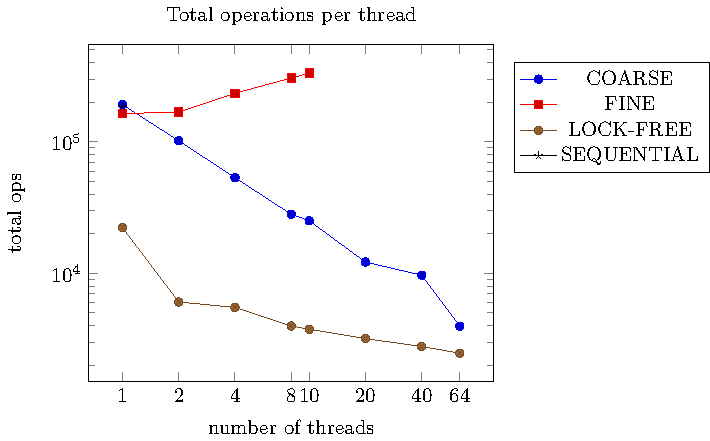
\includegraphics{../plots/parameters2_5s_per_thread.pdf}
        \caption{Configuration parameters2 TOPS per thread,5s execution time}
       
        \label{fig:parameters2_5s_per_thread}
    \end{figure}

    \begin{figure}[H]
        \centering
        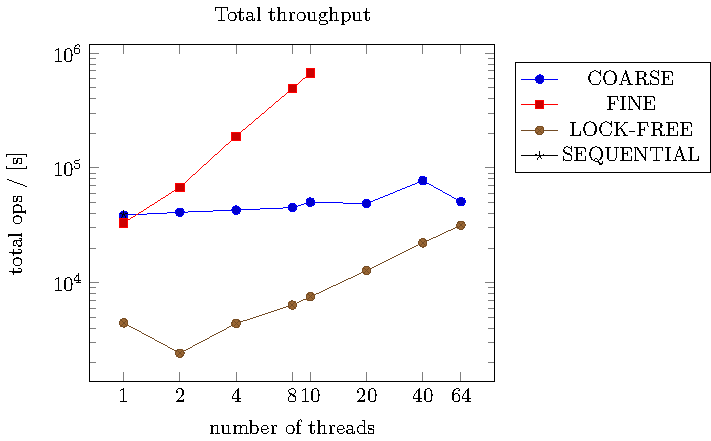
\includegraphics{../plots/parameters2_5s_throughput.pdf}
        \caption{Configuration parameters2 Throughput, 5s execution time}
        \label{fig:arameters2_5s_throughput}
    \end{figure}

The comparative plots show how the different implementations perform on the same input parameters. 
What becomes clear is that the coarse lock implementation does not gain any performance with a higher thread count over a sequential skip list operating on only one thread. 
Also the harsh costs of the atomic operations for the lock-free implementations is obvious. The lazy skip list shows similar scaling with thread count to the lock-free one.


\end{document}
